\section{Investigación previa}

\subsection{La Transformada de Fourier Discreta}

La DFT de una señal discreta $x[n]$, de longitud $N$, está definida como:

\begin{equation}
    X[k] = \sum_{n=0}^{N-1} x[n] \cdot e^{-j \frac{2\pi}{N}kn}, \quad k = 0, 1, ..., N-1
\end{equation}

El cálculo directo de esta fórmula requiere $\mathcal{O}(N^2)$ operaciones complejas.

\subsubsection{La Transformada de Fourier Rápida (FFT)}
\paragraph{Idea general del algoritmo Cooley-Tukey:}

El algoritmo Cooley-Tukey se basa en el paradigma \textit{divide and conquer}, y divide la DFT de tamaño $N$ (donde $N$ es potencia de dos, es decir, $N=2^m$) en dos DFTs de tamaño $N/2$:

\begin{itemize}
    \item Una que contiene los elementos en posiciones pares: $x[0], x[2], x[4], \dots$
    \item Otra con los elementos en posiciones impares: $x[1], x[3], x[5], \dots$
\end{itemize}

Utilizando esta separación, se puede reescribir la DFT como:

\begin{equation}
    X[k] = \sum_{n=0}^{N/2 - 1} x[2n] \cdot W_N^{2kn} + \sum_{n=0}^{N/2 - 1} x[2n+1] \cdot W_N^{(2n+1)k}
\end{equation}

donde $W_N = e^{-j\frac{2\pi}{N}}$ es la raíz $N$-ésima de la unidad.

Agrupando términos:

\begin{equation}
    X[k] = E[k] + W_N^k \cdot O[k]
\end{equation}
\begin{equation}
    X[k + N/2] = E[k] - W_N^k \cdot O[k]
\end{equation}

donde $E[k]$ es la FFT de los elementos pares y $O[k]$ la FFT de los impares. Esta descomposición se aplica recursivamente hasta que se obtienen DFTs de tamaño 1.

\paragraph{Etapas del algoritmo Radix-2:}

\begin{enumerate}
    \item \textbf{Bit-reversal:} Reordenamiento de los datos de entrada según el orden inverso de los bits del índice binario.
    \item \textbf{Cálculo en etapas:} Se realizan $\log_2 N$ etapas, cada una combinando pares de subproblemas más pequeños usando operaciones llamadas \textit{butterflies}.
    \item \textbf{Butterfly operation:} Para cada par $(a, b)$ y una raíz $W_N^k$, se computa:
          \begin{equation}
              a' = a + W_N^k \cdot b, \quad b' = a - W_N^k \cdot b
          \end{equation}
\end{enumerate}

\paragraph{Complejidad computacional:}

Gracias a esta estructura recursiva, el algoritmo tiene una complejidad de:
\begin{equation}
    \mathcal{O}(N \log_2 N)
\end{equation}
lo que representa una mejora sustancial con respecto a la DFT directa.

\paragraph{Ejemplo para $N=4$:}

Sea $x = [x_0, x_1, x_2, x_3]$, se procede como sigue:

\begin{itemize}
    \item FFT de pares: $E[k] = x_0 + x_2 \cdot W_2^k$
    \item FFT de impares: $O[k] = x_1 + x_3 \cdot W_2^k$
\end{itemize}

\noindent Combinación:
\begin{equation}
    X[0] = E[0] + W_4^0 \cdot O[0], \quad X[1] = E[1] + W_4^1 \cdot O[1]
\end{equation}
\begin{equation}
    X[2] = E[0] - W_4^0 \cdot O[0], \quad X[3] = E[1] - W_4^1 \cdot O[1]
\end{equation}

\subsection{Qué es y cómo funciona la transmisión y recepción con Amplitud Modulada (AM)}
La modulación AM es una técnica de transmisión de datos que basa su funcionamiento en encriptación de información como modificaciones de amplitud de ondas de radio.

La modulación es el proceso en el cual se combina una señal de baja frecuencia (información) con una portadora de alta frecuencia para que pueda ser transmitida. Es así como se toma una señal portadora y se modifica su amplitud en base a las variaciones de la onda que se desea enviar. Esto da como resultado la misma onda portadora, pero con variaciones de amplitud en sus extremos superiores e inferiores que contienen la información.

Es así como la transmisión de información involucra la generación de una onda portadora, la modulación de la información en esta portadora, la eventual amplificación de esta señal y por último la transmisión de la onda a través de una antena.

En contraposición, la demodulación es el proceso de extraer la señal moduladora de la señal portadora. Este ejercicio puede abordarse de diversas formas, pero aquí trataremos con la de detección de envolvente. Este método es utilizado cuando trabajamos con señales con un índice de modulación $m \leq 1$ y consiste en rectificar un la onda de entrada, dejando solo el lado positivo y luego seguir la envolvente de la portadora, que efectivamente corresponde a la señal moduladora original.

De este modo, la recepción de una señal consiste en recibir una onda a través de una antena, rectificar usualmente a valores solo positivos, para finalmente filtrar para eliminar los elementos de alta frecuencia comúnmente de la portadora, dejando así una salida que corresponde a la señal moduladora original.

El índice de modulación es una medida de la variación de la amplitud de la onda portadora. Visto de otro modo, se ve como la variación introducida en una portadora por la modulación y se define como $m = \frac{A_m}{A_c}$, donde $A_m$ es la amplitud de la señal de modulación y $A_c$ la amplitud de la señal portadora. Dada la razón m siempre tomará valores positivos o 0, donde: $m=0$ equivale a una portadora no modulada o una moduladora sin información. $0<m<1$ equivale a una portadora submodulada. Esto quiere decir que no se utilizó el total de la portadora para modular, pero sus consecuencias no son tan significativas más allá de un desaprovechamiento de potencial. $m=1$ equivale a una modulación ideal, donde se utiliza todo el potencial de la portadora, variando su amplitud desde su máximo hasta 0. Finalmente $m>1$ es una portadora sobremodulada, lo que resulta problemático dado que hay puntos en que la amplitud de la moduladora se invierte, dando una envolvente invertida la que es difícil de demodular e introduciendo distorsiones en la señal que se quiere transmitir.

\begin{figure}[ht!]
    \centering
    \begin{minipage}{0.48\linewidth}
        \centering
        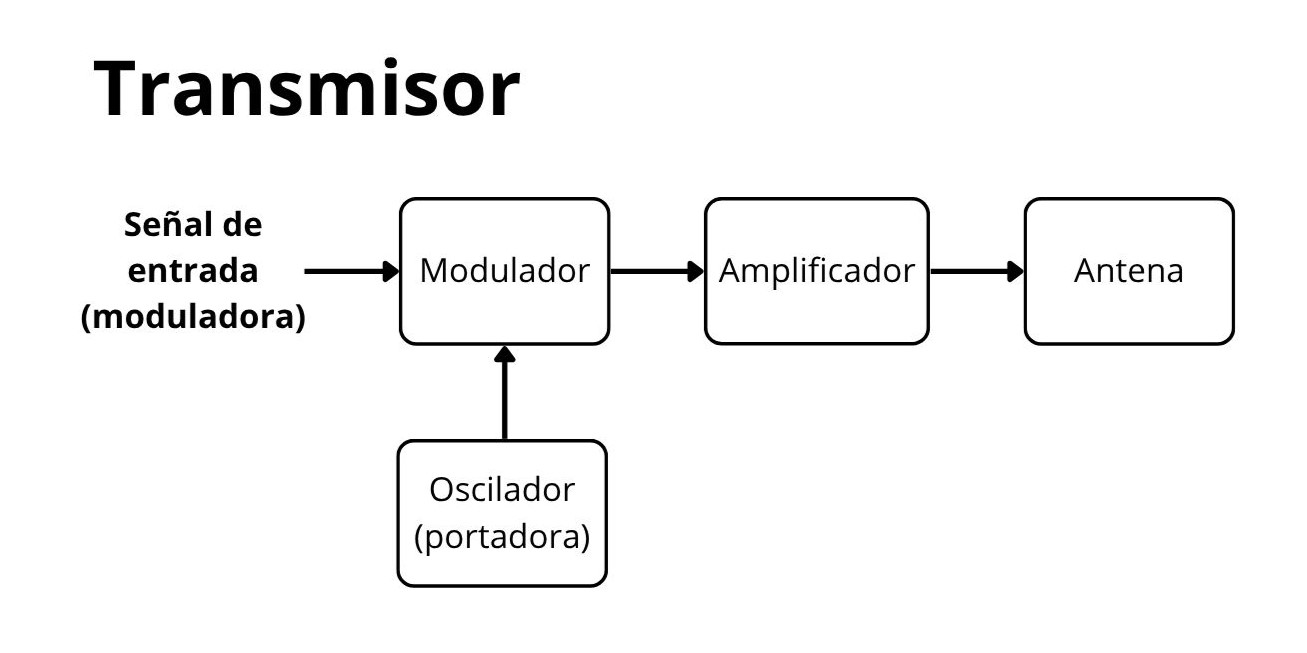
\includegraphics[width=0.95\linewidth]{img/transmisor.jpg}
        \caption{Diagrama de bloques transmisor}
        \label{fig:bloques_transmisor}
    \end{minipage}\hfill
    \begin{minipage}{0.48\linewidth}
        \centering
        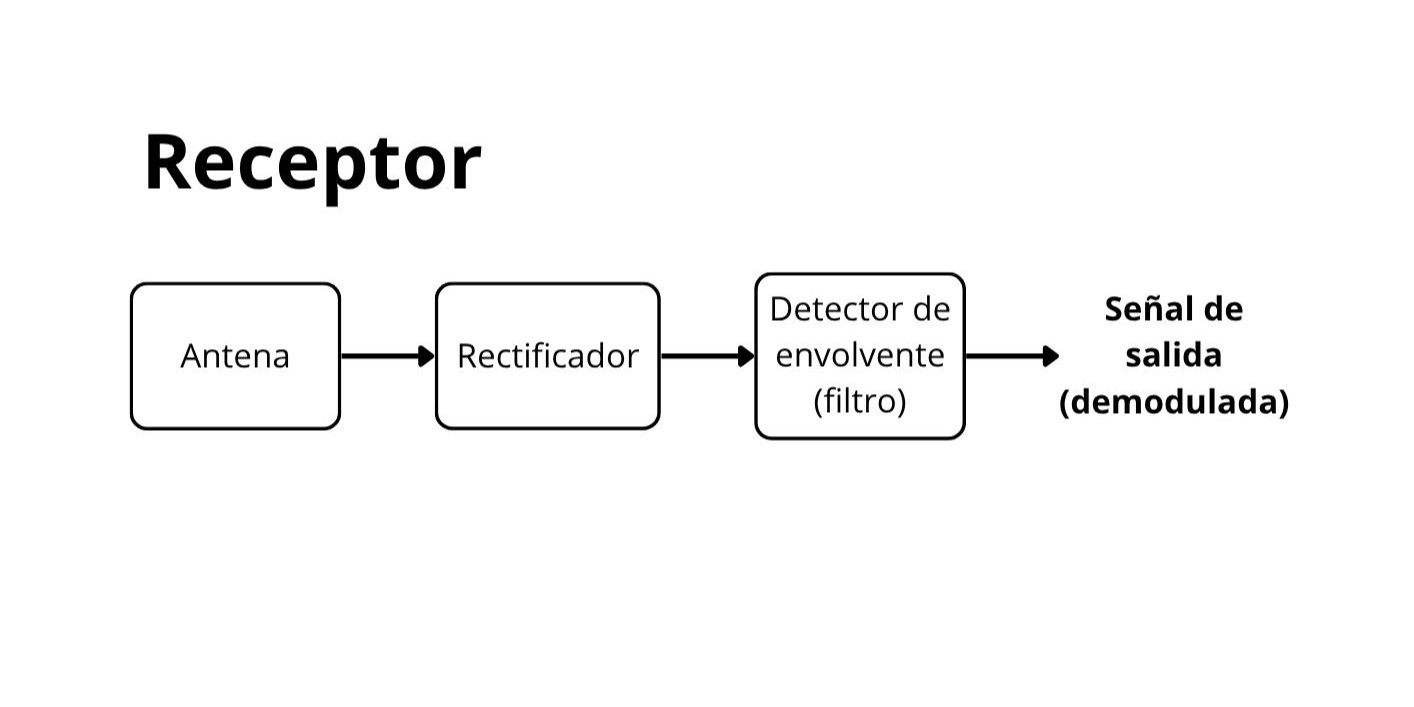
\includegraphics[width=0.95\linewidth]{img/receptor.jpg}
        \caption{Diagrama de bloques receptor}
        \label{fig:bloques_receptor}
    \end{minipage}
\end{figure}

\subsection{Modulación AM Tono Puro}

MOYANO

\subsection{Circuitos de Modulación y Demodulación AM}

\subsubsection{Moduladores AM}
Hay diversas formas de lograr una modulación AM, como el circuíto que se analizará, y tienen la característica de que la señal entrante será la envolvente de otra sinusoide. Otro ejemplo es el siguiente circuíto.

\begin{figure}[htbp]
    \centering
    \begin{circuitikz}[american]

        \draw (0,2) to[sV, l=$V_{in}$] (0,0);

        \draw (0,2) to[D*, l=D] (2,2);

        \draw (2,2) -- (3,2);
        \draw (0,0) -- (3,0);

        \draw (3,2) to[L, l=L, *-*] (3,0);

        \draw (3,2) -- (5,2);
        \draw (5,2) to[C, l=C, *-*] (5,0);
        \draw (5, 0) -- (3, 0);

        \draw (5,2) to[short, -*] (6,2);
        \draw (6,2) node[right]{$V_{AM}$};
    \end{circuitikz}
\end{figure}

Aquí la señal entrante $V_{in}$ será la envolvente de la señal $V_{AM}$, que será la que viajará.

\subsubsection{Demoduladores AM}

Los circuítos demoduladores AM tienen que conseguir la información de la envolvente, por lo que un ejemplo de esto son los rectificadores, que recordando, considera los picos de la sinusoide, por lo que en nuestro contexto, lo que se recupera será la envolvente. Un ejemplo de circuíto demodulador AM es:

\begin{figure}[htbp]
    \centering
    \begin{circuitikz}[american]

        % Fuente de señal AM
        \draw (0,0) to[sV, l=$V_{AM}$] (0,3);

        % Diodo
        \draw (0,3) to[short] (1,3)
        to[D*, l_=D] (2,3);

        % Nodo superior del RC
        \draw (1,3) -- (3,3);

        % Condensador hacia abajo
        \draw (3,3) to[C, l_=C] (3,0);

        % Resistencia hacia derecha
        \draw (3,3) to[short] (5,3)
        to[R, l = R] (5,0);

        % Cable inferior de masa
        \draw (0,0) -- (5,0);
        \draw (5,3) to[short, -*] (6,3);
        \draw (6, 3) node[right]{$V_{out}$};

    \end{circuitikz}
\end{figure}

En particular, la radio galena es un ejemplo simple y económico de un demodulador AM que además, tiene la misma forma que el circuíto mostrado. En este caso, el voltaje AM es recibido por una antena y transmitido por un transformador que amplifica la señal, y la resistencia corresponde al audífono con el que escuchamos la señal de radio.

\subsubsection{Espectro de frecuencia}

Para entender esto, hay que recordar cómo se ve una onda con modulación AM:

\begin{equation*}
    V_{AM}=V_{in}(1+m\cos(\omega_mt))\cos(\omega_{in}t)
\end{equation*}

donde m es el indice de modulación. Dado esto, se puede encontrar una nueva expresión para esta onda:

\begin{align*}
    V_{AM} & =V_{in}\cos(\omega_{in}t)+mV_{in}\cos(\omega_mt)\cos(\omega_{in}t)                                        \\
    V_{AM} & =V_{in}\cos(\omega_{in}t)+\frac{1}{2}mV_{in}[\cos([\omega_m+\omega_{in}]t)+\cos([\omega_m-\omega_{in}]t)]
\end{align*}

De esta manera, se pueden identificar 3 ondas, la onda portadora, que es $V_{in}\cos(\omega_{in}t)$ y las ondas de banda lateral superior e inferior, que son aquellas cuya frecuencia queda determinada por $\omega_{sup}=\omega_m+\omega_{in}$ y $\omega_{inf}=\omega_m - \omega_{in}$ respectivamente. De esta manera, se puede determinar el ancho de banda de una onda modulada, que queda determinado por $BW = \omega_{sup}-\omega_{inf} = 2\omega_m$.

\subsubsection{Tecnologías actuales que usan AM}

Actualmente, las tecnologías que usan AM son bastante cotidianas, y se presentan en varias formas, como en el wifi, la comunicación por cable y por satélite, las redes móviles, la radio AM o la televisión.

\subsubsection{Radiofusión AM utilizada en Chile y el espectro audible}

La radiodifusión AM modula sonido en la amplitud de ondas de radio, sin embargo, las radios actuales prefieren la modulación FM, pues su calidad de audio y resistencia al ruido son mayores. Las radios actuales que usan la modulación AM en Chile usan un rango de frecuencias entre los 540 y los 1610KHz.